\chapter{Related Work / Program Synthesis}\label{chap:program-synthesis}


Program synthesis is a very wide field of research. It has been studied by different research communities and applied to diverse problems. As such, many approaches have been proposed to deal with the specific challenges introduced by each application, resulting in a great variety of focused algorithms that aim at finding a better program in less time. In this section, we take a more in-depth look into some of these techniques.

In \autoref{sec:cegis}, we look at a way to steer the search in the right direction by using information about wrong answers to avoid future similar mistakes. In sections~\ref{sec:ogis} and~\ref{sec:user-interaction}, we look at different ways to deal with the ambiguity of the desired behaviour specification in inductive synthesis.

Finally, in \autoref{sec:synth-predicates}, we take an in-depth look at \textit{AlphaRegex}, a tool that, though not directly addressing the form validation problem, tackles the synthesis of regular expressions, which are an important part of our domain.

\section{Sketch-based Enumerative Search}
\begin{figure}
    \centering
    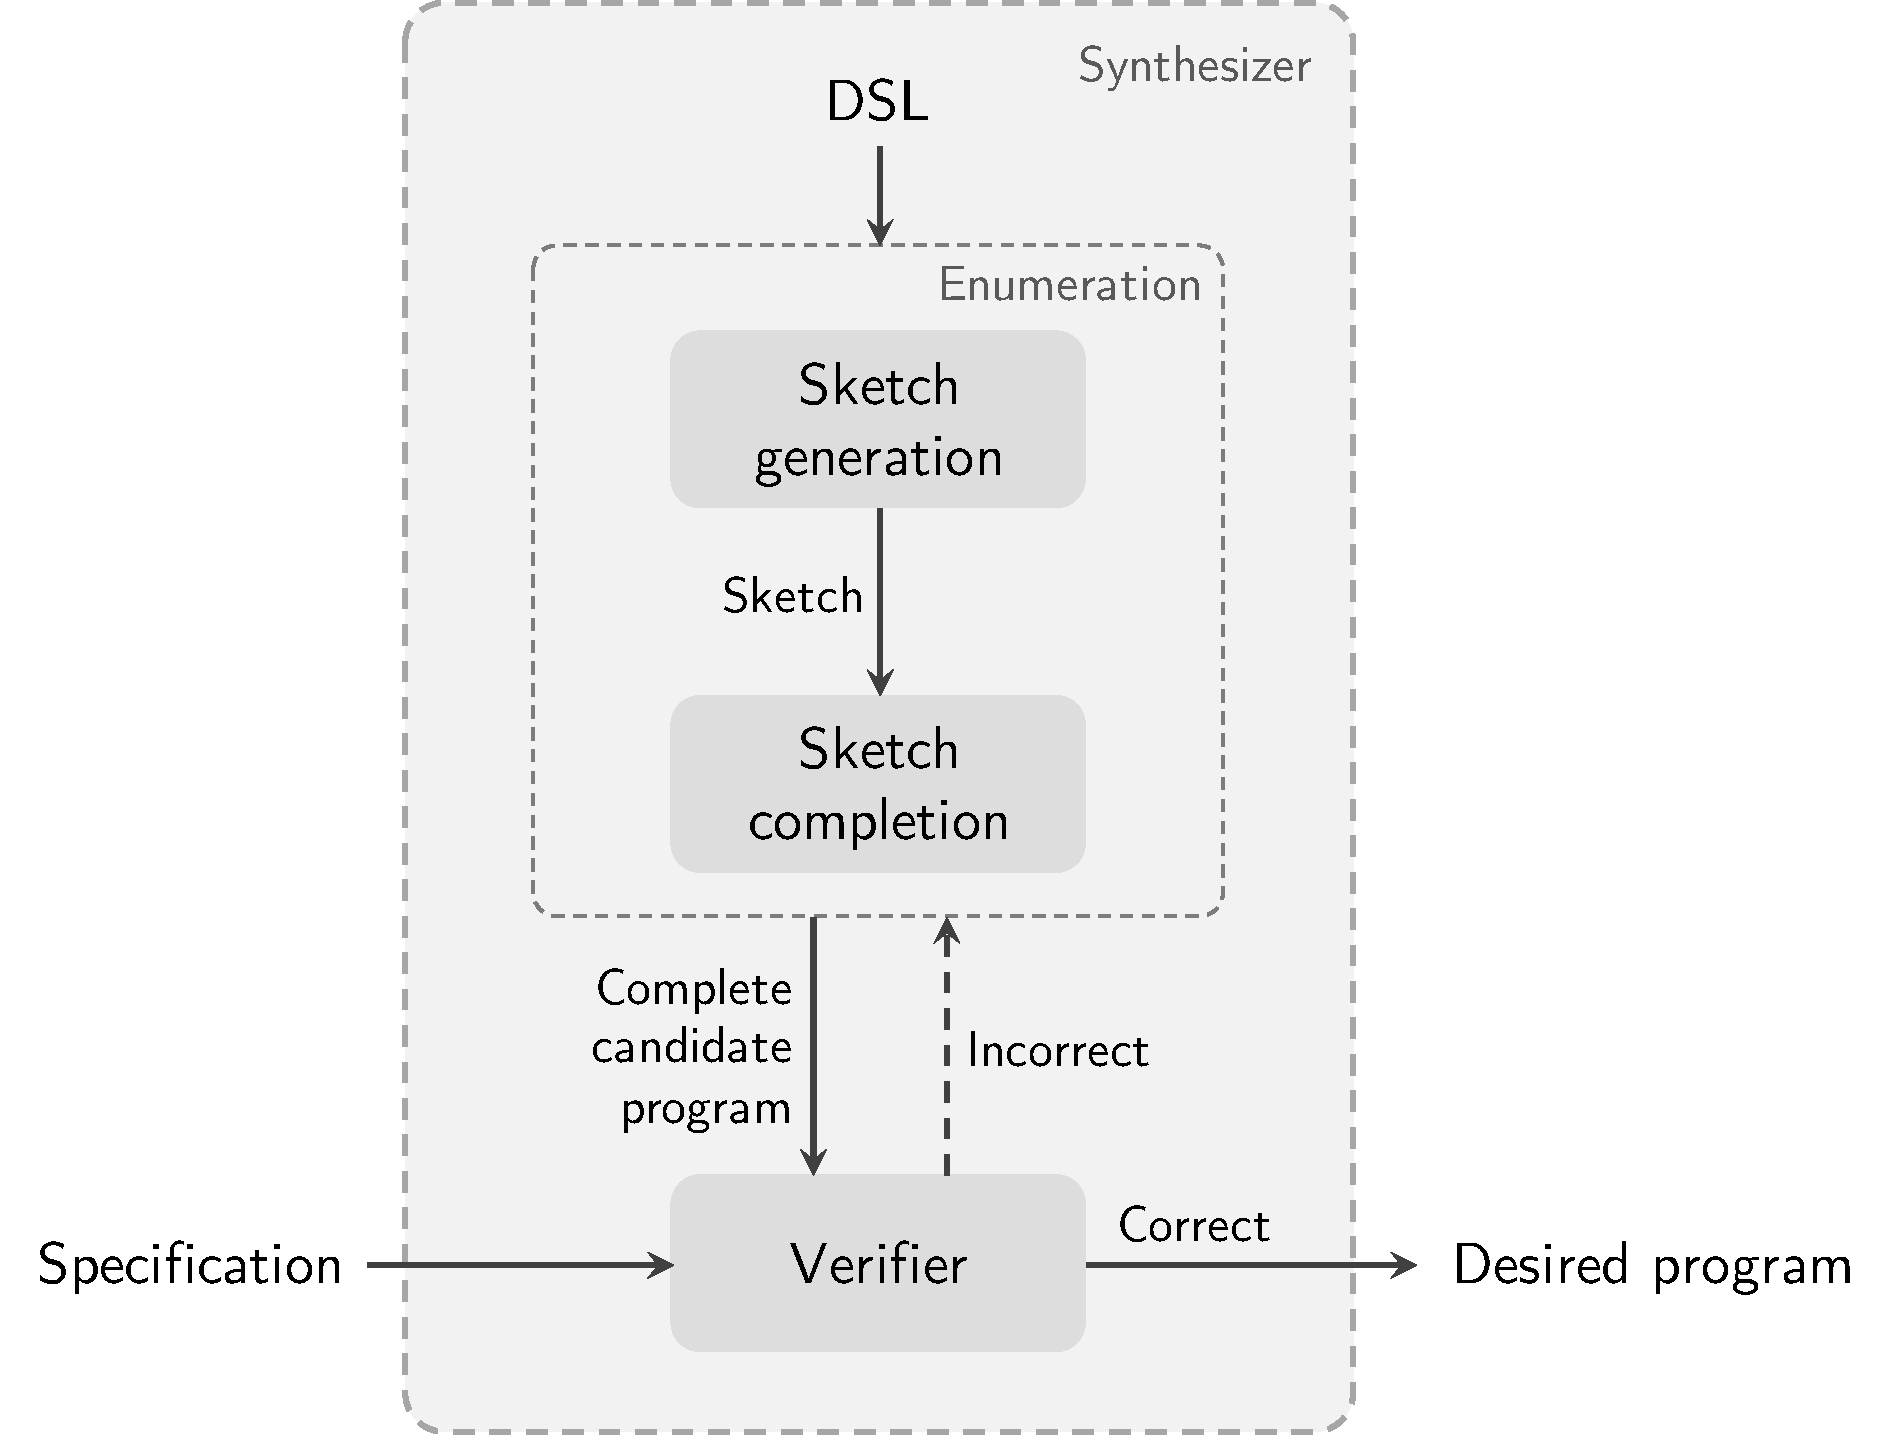
\includegraphics[scale=.35]{pictures/sketch.pdf}
    \caption{Sketch-based enumeration}
    \label{fig:sketch_enumeration}
\end{figure}
Some synthesizers opt to perform enumerative search using partial programs.
Partial programs (often called sketches) are a high-level representation of the intended program. Instead of completely defining a program, they contain holes, i.e., parts of the program that refer to lower-level implementation details. For a sketch to become syntactically correct, all its holes must be filled with syntactically correct expressions.

Instead of enumerating complete programs, a sketch-based synthesizer takes one of two approaches: Either
\begin{enumerate*}[label=(\roman*)]
    \item a sketch is provided by the user, who already possesses a high-level description of the desired program, in which case the synthesizer must complete it according to the specification, or
    \item the synthesizer is responsible for both producing a suitable sketch and completing it. The enumeration process is then split in two steps: sketch generation and sketch completion.
\end{enumerate*}
During sketch generation, the synthesizer enumerates incomplete programs in some order. During sketch completion, the synthesizer then enumerates complete programs for each given sketch, by successively filling each hole with a syntactically correct expression. Sketch-based enumeration is outlined in \autoref{fig:sketch_enumeration}.


\section{\acl{CEGIS}}\label{sec:cegis}

Program synthesis is a search problem where the goal is to find a program \(P\) that satisfies a given specification \(\phi\).
\(\phi(\vec{x}, y)\) is \true{} if and only if \(y\) is the desired output value for input \(\vec{x}\).
We can define the program synthesis problem with the following logic formula:
%
\begin{equation}\label{eq:ps-2nd-order}
\exists P \; \forall \vec{x}, y : (P(\vec{x}) = y) \Rightarrow \phi(\vec{x}, y).
\end{equation}
%
\noindent
Due to the existential quantifier over function \(P\), \eqref{eq:ps-2nd-order} is a second-order formula and, as such, it is generally undecidable. 
To work around this problem, we may note that even though \textit{finding} a program that satisfies a specification may be infeasible, \textit{verifying} that a given program \(P\) satisfies a specification is a first-order problem:
%
\begin{equation}\label{eq:ps-1st-order}
\forall \vec{x}, y : (P(\vec{x}) = y) \Rightarrow \phi(\vec{x}, y).
\end{equation}
%
Formula \eqref{eq:ps-1st-order} is a first-order formula and can be solved using an off-the-shelf first-order solver. Any program \(P\) that satisfies~\eqref{eq:ps-1st-order} is a correct program, i.e., it complies with the specification \(\phi\).
Instead of proving \eqref{eq:ps-1st-order}, we can equivalently disprove its negation:
%
\begin{equation}\label{eq:counterexample}
\exists \vec{x}, y : (P(\vec{x}) = y) \wedge \neg \phi(\vec{x}, y).
\end{equation}
%
Formula \eqref{eq:counterexample} is also a first-order formula.
Formula~\eqref{eq:counterexample} is unsatisfiable if and only if \(P\) is a correct program.
Therefore, to find a correct program, we search the program space for a program \(P\) such that~\eqref{eq:counterexample} is unsatisfiable. Once found, \(P\) can be returned to the~user. %To achieve this, we can use enumerative search (previously explained in \autoref{sec:enum-search}), whose definition fits well into this way of verifying correctness of the program: the \textit{verifier} entity is then a solver that tries to satisfy formula~\eqref{eq:counterexample} (see Figures \ref{fig:enumerative-search} and~\ref{fig:CEGIS}).

\begin{figure}
    \centering
    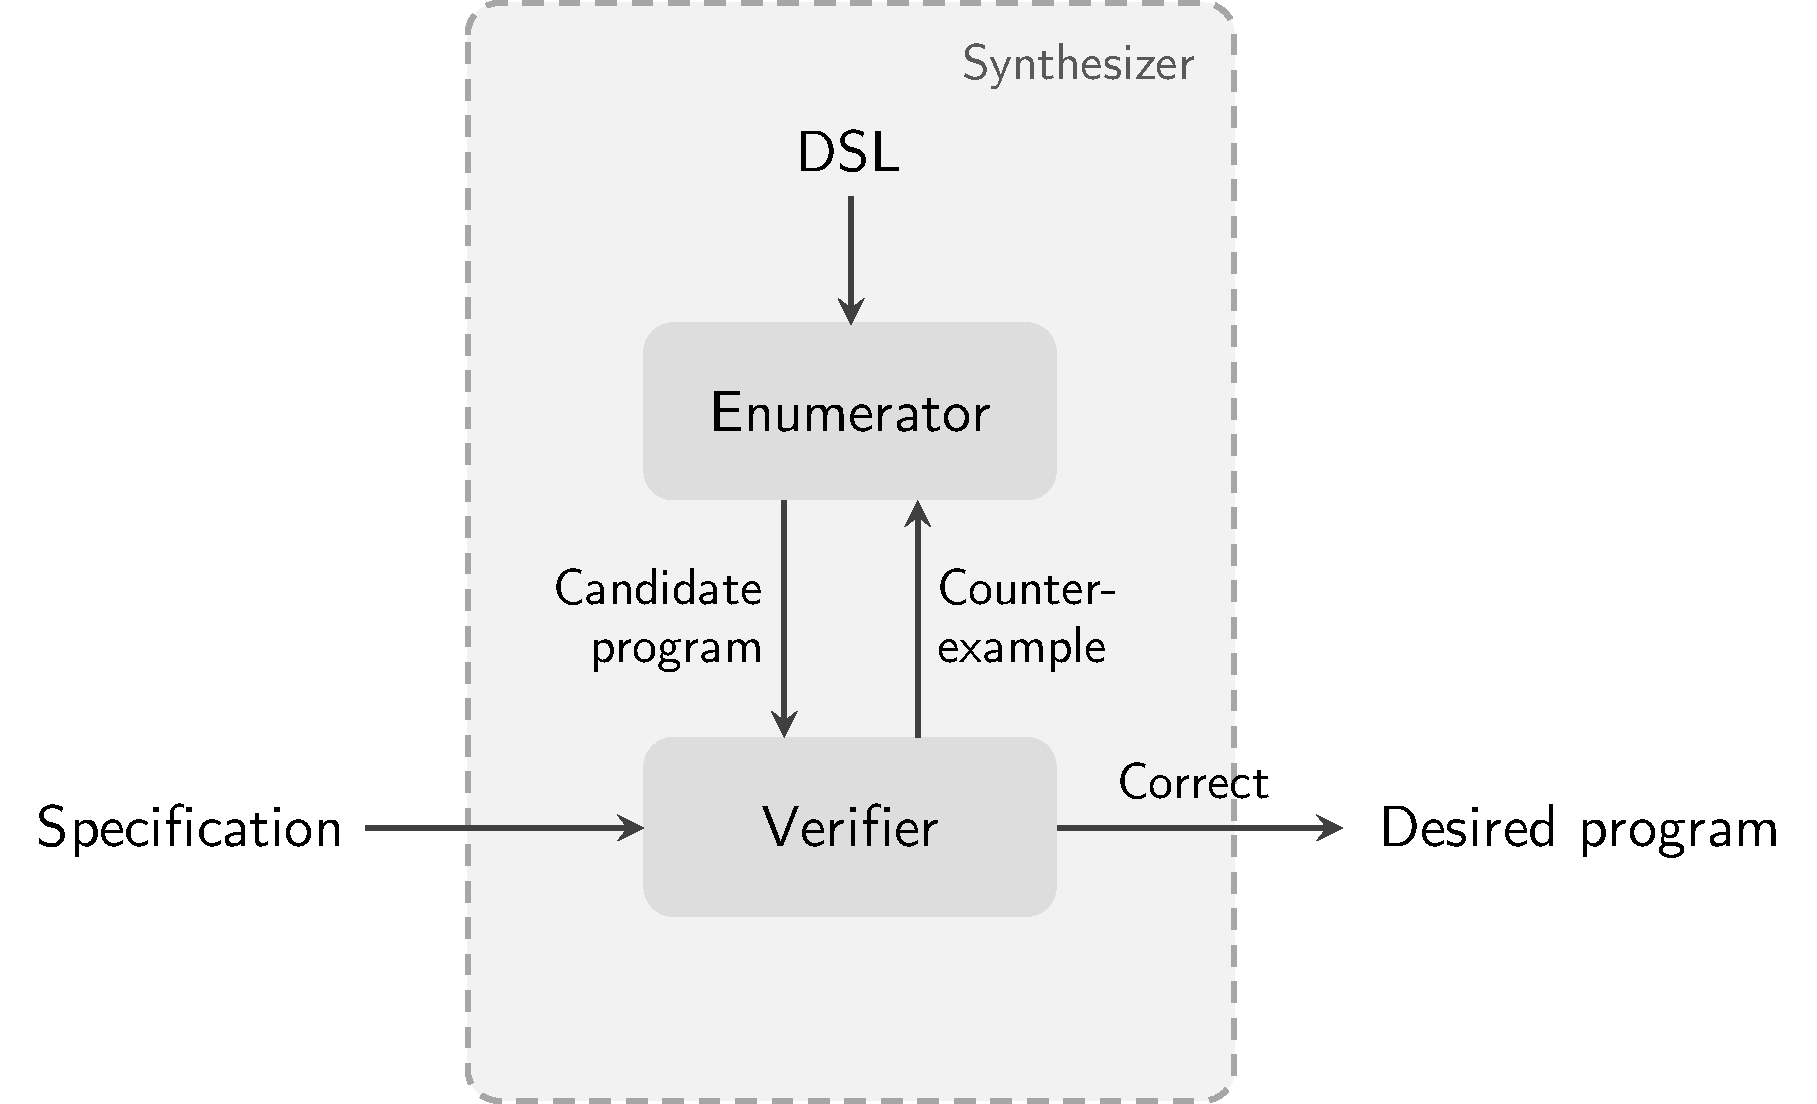
\includegraphics[scale=.35]{pictures/cegis.pdf}
    \caption{\ac{CEGIS}}
    \label{fig:cegis}
\end{figure}

Whenever we encounter a program \(P\) for which formula~\eqref{eq:counterexample} is satisfiable, the values of \(\vec{x}\) and \(y\) that satisfy the formula constitute a counterexample: an input \(\vec{x}\) for which \(P\) does not satisfy the specification \(\phi\); in other words, an input \(\vec{x}\) to which our program returns the wrong output.
If we take this counterexample \((\vec{x}, y)\) into account during our subsequent search, none of the new candidate programs will return \(y\) on the input \(\vec{x}\).
We have thus strengthened the specification, eliminating the previous incorrect candidate program.

\begin{definition}[Counterexample]
A counterexample \((\vec{x}, y)\) for an incorrect program \(P\) is an input-output pair such that \(P(x) = y\) and \(\neg \phi(\vec{x}, y)\), i.e., \(y\) is the output returned by \(P\) on input \(\vec{x}\) even though \((\vec{x}, y)\) is not consistent with the specification.
\end{definition}

This approach was proposed in \citeyear{Solar-LezamaPhDThesis} by \citeauthor{Solar-LezamaPhDThesis} in his PhD Thesis \cite{Solar-LezamaPhDThesis} and it is represented in \autoref{fig:cegis}. In this figure, the \textit{verifier} is a solver that tries to satisfy formula~(\ref{eq:counterexample}).

We can further improve this method by reformulating the verification formula in order to produce a constructive counterexample:
%
\begin{equation}\label{eq:constructive}
\exists \vec{x}, y : (P(\vec{x}) \neq y) \wedge \phi(\vec{x}, y).
\end{equation}
%
Like before, \eqref{eq:constructive} is a first-order formula and it is unsatisfiable if and only if \(P\) is a correct program.
When \eqref{eq:constructive} is satisfiable \(P\) is not a correct program and the values of \(\vec{x}\) and \(y\) that satisfy the formula are now a \textit{constructive} counterexample: \(y\) is the correct output for input \(\vec{x}\).
While a model \((\vec{x}, y)\) that satisfies \eqref{eq:counterexample} is an input-output pair that the program must \textit{not} satisfy, a model \((\vec{x}, y)\) that satisfies \eqref{eq:constructive} is a correct input-output pair that the program \textit{must} satisfy.
Adding the constructive counterexample to our previous specification results in a much stronger constraint and prunes the remaining search space even further. %However, this reformulation is only possible when there is only one output value that satisfies the specification for the input value~\(\vec{x}\).

\begin{definition}[Constructive counterexample]
A constructive counterexample \((\vec{x}, y)\) for an incorrect program \(P\) is an input-output pair such that {{\(P(x)~\neq~y\)}} and \(\phi(\vec{x}, y)\), i.e., \(y\) is not the output returned by \(P\) on input \(\vec{x}\) even though \((\vec{x}, y)\) is consistent with the specification.
\end{definition}

\section{\acl{OGIS}} \label{sec:ogis}
As discussed in \autoref{sec:desired-behaviour-spec}, \ac{PBE} comes with the drawback of incompleteness of the behaviour specification. Many programs are consistent with the provided specification, but not all these programs exhibit the user's intended behaviour.

In order to restore soundness of the solution, \citeauthor{DBLP:conf/icse/JhaGST10} proposed in \citeyear{DBLP:conf/icse/JhaGST10} a new approach which makes use of distinguishing inputs to disambiguate the input-output examples: \acf{OGIS}~\cite{DBLP:conf/icse/JhaGST10}.
An \textit{I/O~oracle} maps any given input to the desired output and it is used as an alternative to a complete specification. This means that whenever the \textit{I/O~oracle} is queried on any input vector \(\vec{x}\), it always returns the correct output \(y\).

We start with the same schema we had for \ac{CEGIS} (\autoref{fig:cegis}),  with a \textit{verifier} which, upon receiving a program \(P\), decides whether it is consistent with the behavioural constraints~\(\phi\). However, in \ac{OGIS} we no longer return to the user the first correct program we find.

When a correct program \(P_1\) is found, it is stored, and the search continues for another correct program. If no other correct program is found, then \(P_1\) is the unique correct program and it can be returned to the user. If another correct program \(P_2\) is found, then we have two programs consistent with the provided specification, i.e., \(P_1\) and \(P_2\) satisfy the following formulas:
%
\begin{subequations}
\begin{equation}
  \forall \vec{x}, y : (P_1(\vec{x}) = y) \Rightarrow \phi(\vec{x}, y),
\end{equation}
\begin{equation}
  \forall \vec{x}, y : (P_2(\vec{x}) = y) \Rightarrow \phi(\vec{x}, y).
\end{equation}
\end{subequations}

\noindent
Upon finding two correct programs, we want to find an input to which the two programs \(P_1\) and \(P_2\) return different outputs: a \textit{distinguishing input}. To produce a distinguishing input, we can try to solve:
%
\begin{equation}\label{eq:distinguishing}
  \exists \vec{x}, y_1, y_2: P_1(\vec{x}) = y_1 \wedge P_2(\vec{x}) = y_2 \wedge y_1 \neq y_2.
\end{equation}
%
If formula~(\ref{eq:distinguishing}) is unsatisfiable then \(P_1\) and \(P_2\) are equivalent programs.
In this case, either there are more correct programs that can be taken into consideration, or \(P_1 = P_2\) is the unique program that satisfies all input-output examples and it is returned to the user.
If~(\ref{eq:distinguishing}) is satisfiable, the distinguishing input \(\vec{x}\) can be extracted from the model \((\vec{x}, y_1, y_2)\) that satisfies it.
Once found, we can query the \textit{I/O oracle} on the distinguishing input, who yields the correct output for it.
The distinguishing input along with its correct output forms a new correct input-output pair \((\vec{x}, y)\) which can then be added to the specification~\(\phi\), further constraining the search space.

In the end of this cycle, we have a set of input-output pairs that completely specify the generated program, thus eliminating all ambiguity.

\begin{figure}
    \centering
    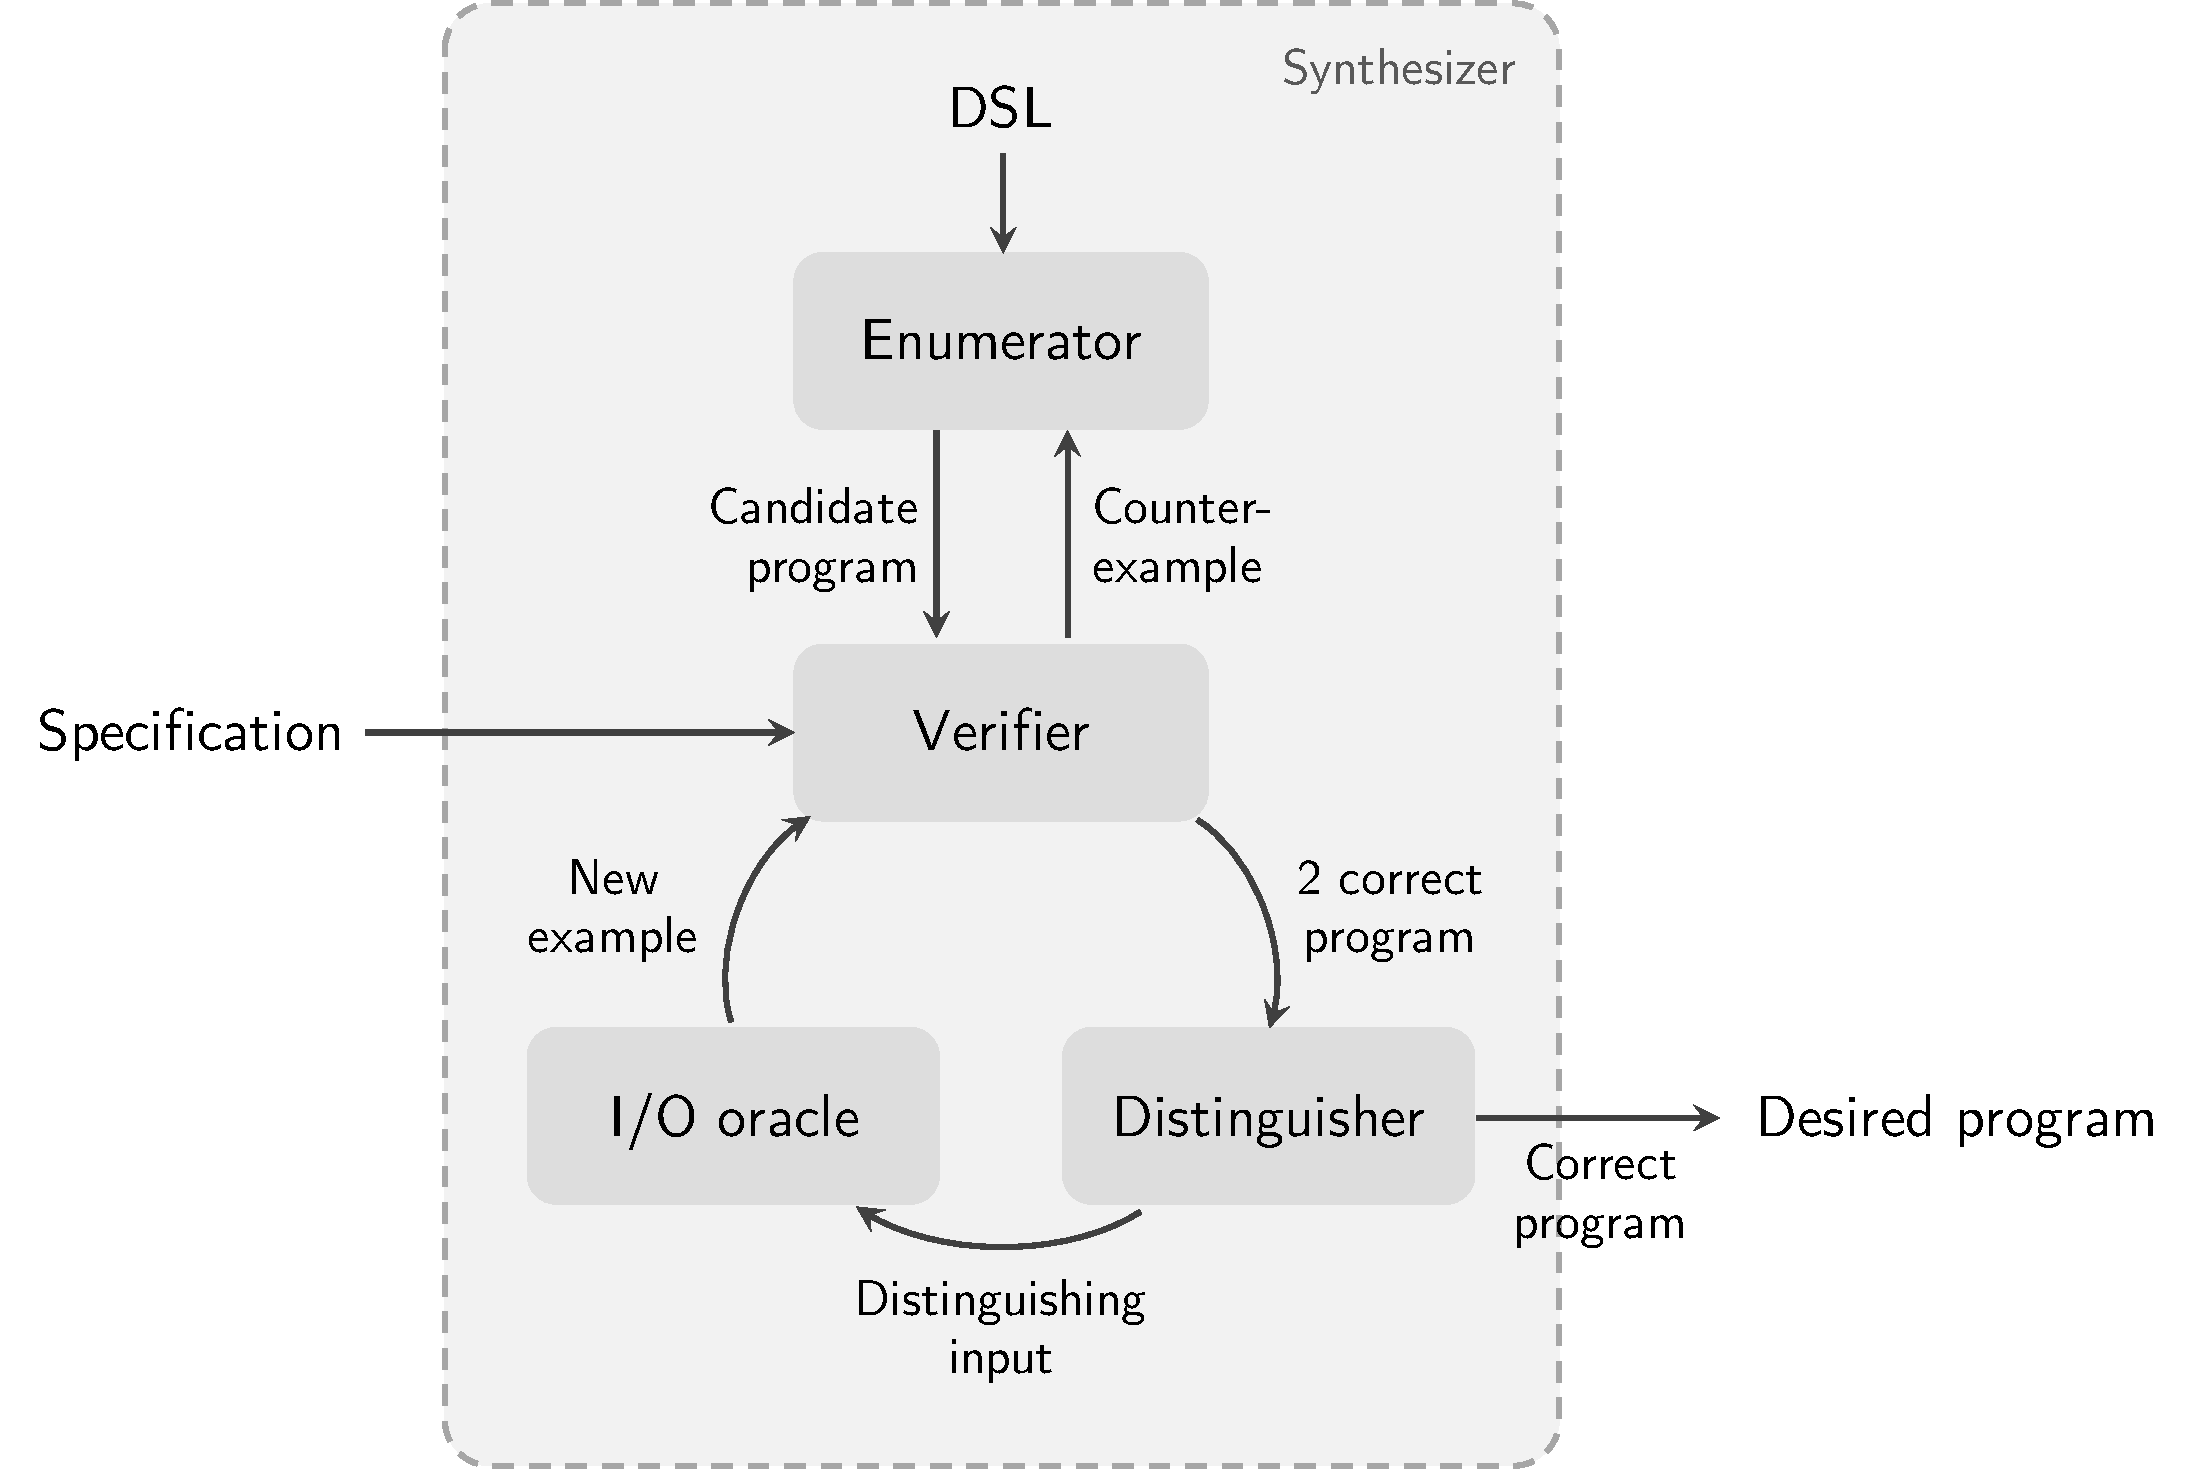
\includegraphics[scale=.35]{pictures/ogis.pdf}
    \caption{\ac{OGIS}}
    \label{fig:ogis}
\end{figure}

This method is illustrated in \autoref{fig:ogis}. In this figure, the \textit{enumerator} and \textit{verifier} are identical to those in \ac{CEGIS} (\autoref{fig:cegis}). The \textit{distinguisher} is a new entity, which can be a solver that tries to satisfy formula~(\ref{eq:distinguishing}).


\section{User Interaction} \label{sec:user-interaction}

As mentioned before, \ac{PBE} uses input-output examples as the desired behaviour specification, which can be very ambiguous. When the synthesizer simply picks a correct program to return to the user, it may not satisfy the desired behaviour in corner cases not covered by the examples provided.
In order to increase confidence in the synthesizer's solution, a good way to disambiguate the specification is by explicitly interacting with the user so he or she can provide further information about the intended~program.
% In this section we look at two different user interaction models that allow the synthesizer to gather more information about the intended program, thus resolving the ambiguity in the initially provided examples.

\subsection{Conversational Clarification}
\begin{figure}
    \centering
    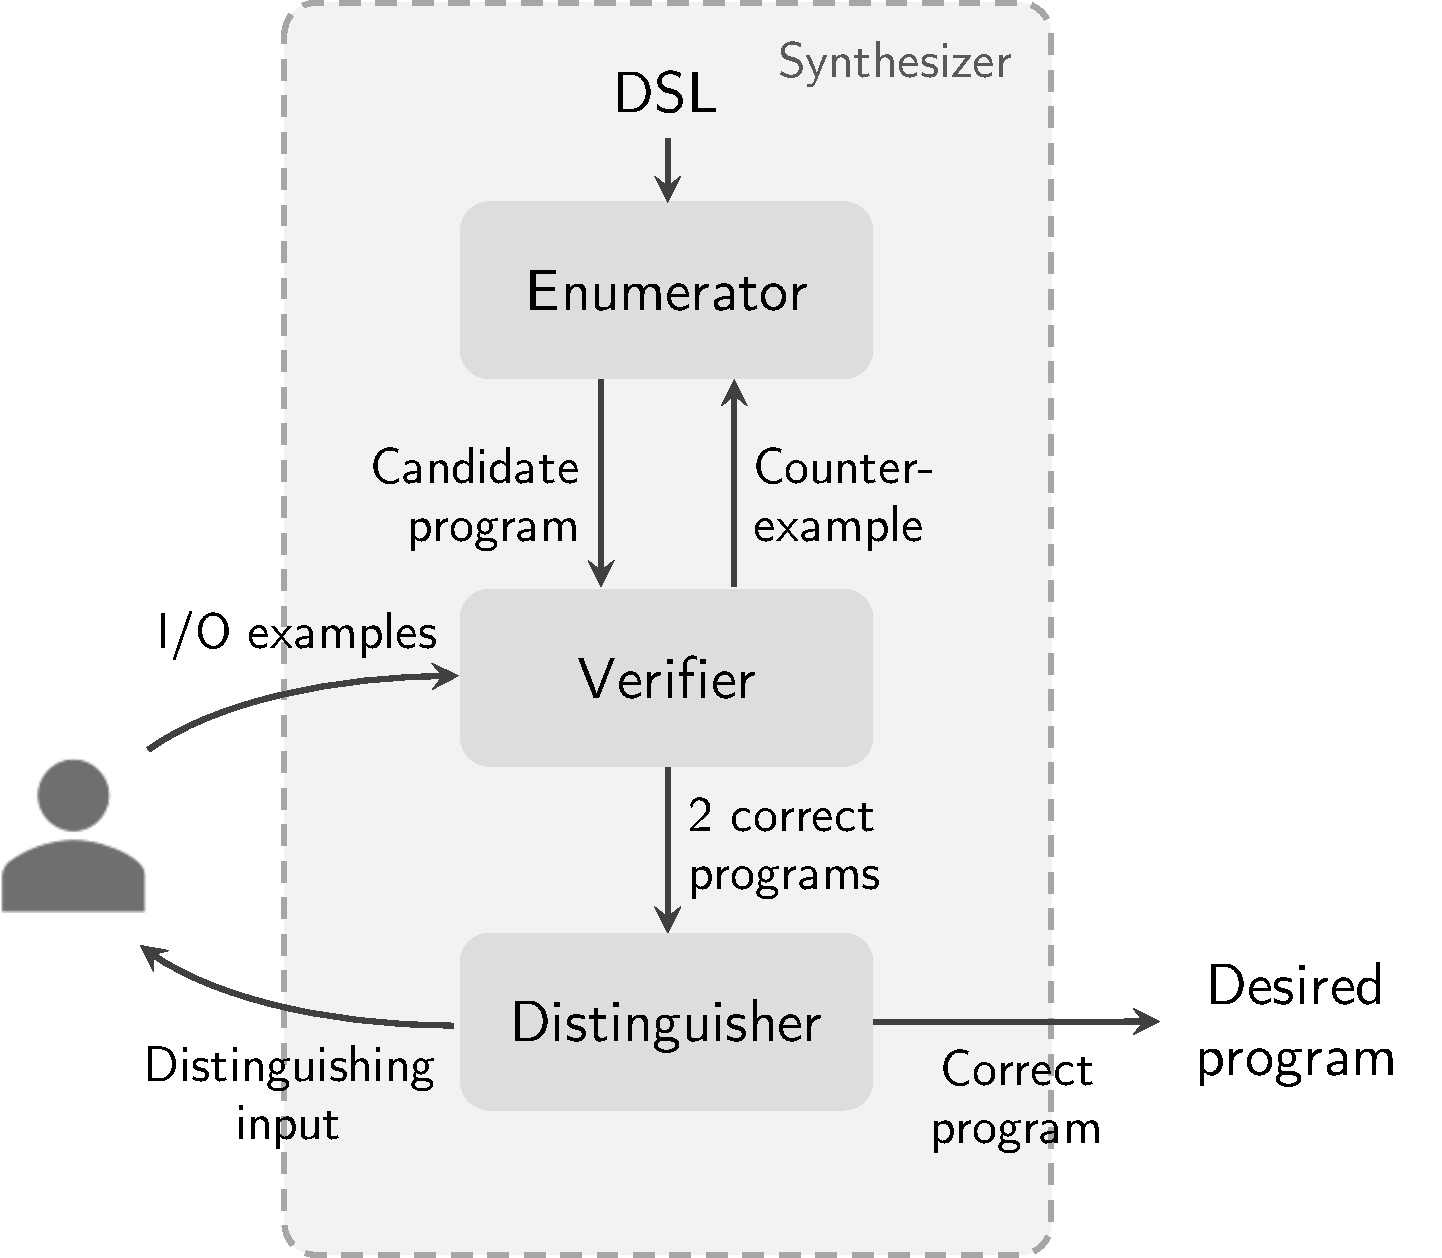
\includegraphics[scale=.35]{pictures/conversational_clarification.pdf}
    \caption{Conversational clarification}
    \label{fig:conversational_clarification}
\end{figure}

Conversational clarification is an interaction method described by \citeauthor{DBLP:conf/uist/MayerSGLMPSZG15} \cite{DBLP:conf/uist/MayerSGLMPSZG15} which has been successfully used in many synthesizers  \cite{DBLP:journals/pvldb/LiCM15,DBLP:journals/corr/abs-19,DBLP:conf/sigmod/WangCB17,DBLP:conf/pldi/WangCB17}.
During the synthesis procedure, the synthesiser asks questions to the user with respect to certain inputs, and uses the answers to resolve ambiguities in the desired behaviour specification. 

After the synthesizer has generated several programs that are consistent with the user-provided examples, it uses the \textit{distinguisher} described in \autoref{sec:ogis} to produce a distinguishing input: an input for which two correct programs yield two different outputs. The synthesizer then queries the user on what is the desired output for that specific input (it may be the output returned by one of the synthesised programs, or a different one altogether). The distinguishing input along with the desired output form a new input-output example, which is added to the specification, making it stronger. Each distinguishing input splits the search space in a different way, so the number of necessary user interactions depends on the chosen distinguishing input in each iteration. In the end, only one program remains. Since all ambiguity in the original specification has been resolved, the remaining program is the desired program and it can be returned to the user.

Conversational clarification is represented in \autoref{fig:conversational_clarification}. It is no more than a variation of the \ac{OGIS} method, described in \autoref{sec:ogis}, where the user plays the part of the \textit{I/O oracle}.


\subsection{Ramos's Interaction Models}

\citet{UnchartIt} propose two interaction models: \textsc{Options} and Y/N. Both models interact with the user using distinguishing inputs, i.e., new inputs generated by the synthesizer that allow

\todo{Explain}

\section{Regex synthesizers}\label{sec:related-work}



\subsection{\textit{AlphaRegex}}
\label{sec:synth-predicates}
In \citeyear{AlphaRegex16}, \citet{AlphaRegex16} presented \textit{AlphaRegex}, a \ac{PBE} synthesizer of regular expressions in the binary alphabet, \(\Sigma = \{0, 1\}\).

To use \textit{AlphaRegex}, the user describes the desired accepted language by providing a set of positive and negative examples. The synthesised regular expression must define a language that includes all the positive examples and none of the negative ones.
\textit{AlphaRegex} uses an enumerative search technique, with a ranking method that prioritises simpler expressions.

The algorithm starts by examining the simplest regular expressions, \regex{0} and \regex{1}.
If these are not consistent with the examples, it checks more complex productions such as \regex{0|0}, \regex{0|1}, \regex{1|0}, \regex{1|1} (i.e. expressions in the form of \regex{\Box|\Box}), \regex{00}, \regex{01}, \regex{10}, \regex{11} (i.e. expressions in the form of \(\tt\Box\Box\)), and \regex{0*}, \regex{1*}, (i.e. expressions in the form of \(\tt\Box*\)).

Here, we introduce the hole (\(\Box\)), a placeholder for any regular expression. Regular expressions with or without holes are the states of the search.
The algorithm generates regular expressions by iteratively replacing holes with other states and checking if the resulting regular expressions are correct.

To speed up the search, \textit{AlphaRegex} makes use of three different kinds of search space pruning techniques: over-approximation, under-approximation and elimination of redundant states.

\paragraph{Over-approximation} is achieved by replacing holes in the current state with \regex{(0|1)*}.
This regular expression describes the language that accepts all the strings that can be written using the binary alphabet.
%The union of any  regular expression \(r\) with \regex{(0|1)*}, \(r|\tt(0|1)*\), is again \regex{(0|1)*}.
%The concatenation of any regular expression \(r\) with \regex{(0|1)*}, \(r\tt(0|1)*\), results in the original regular expression \(r\).
Therefore, over-approximation makes the state as general as it can be.
If the over-approximation rejects at least one of the positive examples we conclude that this state can never be used to build a solution.

\begin{example}
Consider the state \(\tt1\Box\), i.e., the concatenation of \regex{1} with a hole, which can be filled with any regular expression. The over-approximation of this state, \regex{1(0|1)*}, accepts all strings that a regular expression of the form \(\tt1\Box\) could possibly accept. Thus, if \regex{1(0|1)*} does not accept all the the positive examples, this state is not worth considering, and can be pruned.
\end{example}

\paragraph{Under-approximation} consists in replacing holes in the current state with \regex{\emptyset}, the regular expression that corresponds to the empty language. The concatenation of any regular expression \(r\) with \(\tt\emptyset\), \(r\tt\emptyset\), results in \(\tt\emptyset\). The union of any  regular expression \(r\) with \(\tt\emptyset\), \(r|\tt\emptyset\), is the regular expression \(r\) itself.
If the under-approximation does not reject any of the negative examples,  we conclude that this state can never be used to build a correct solution.

\begin{example}
Consider now the state \(\tt1|\Box\), i.e., the union of \regex{1} with a hole. The under-approximation of this state, \(\tt1|\emptyset = 1\), restricts \regex{1|\Box} to the language that accepts as few strings as possible, in this case, the one containing only the string with a single `1'. If \regex{1} does not reject any of the negative examples, then this state can be pruned.
\end{example}

\paragraph{Elimination of redundant states} is done using the equivalences of regular expressions resulting from the algebraic rules of regular expressions.
%  described in \autoref{tab:regex-laws} in \autoref{sec:regex}
For example, the algorithm needs not evaluate the expression \(s\texttt{|}r\) if it has already considered \(r\texttt{|}s\), where \(r\) and \(s\) are regular expressions, as these expressions are equivalent.

\medskip

\noindent
The authors tested \textit{AlphaRegex} in 25 benchmark problems collected from textbooks on automata theory which are provided along with the code for their tool.
\textit{AlphaRegex} proved capable of synthesising relatively complex expressions, with more than a dozen operations, in under one minute.


\subsection{\Regel}

\todo{\Regel!}